This section evaluates the proposed FireRoute system through scenario-based experiments on a controlled campus-scale testbed. The evaluation focuses on how the system responds to operational constraints, environmental perturbations, and infrastructure conditions, as well as its ability to provide interpretable and actionable decision support.

\subsection{Experimental Setup}

\begin{table}[t]
\caption{Pilot package summary for graph, asset, scenario, and governance artifacts.}
\label{tab:assets}
\centering
\scriptsize
\setlength{\tabcolsep}{3.5pt}
\renewcommand{\arraystretch}{0.92}
\begin{tabular}{L{2.25cm} C{0.8cm} L{3.95cm}}
\toprule
Artifact & Count & Notes \\
\midrule
Graph nodes & 21 & Campus stations, road anchors, shelters, and POIs \\
Graph edges & 25 & Main roads, alleys, and footpath connectors \\
Hydrants & 12 & Mixed operational states with health-check metadata \\
Sensors & 3 & Smoke, carbon monoxide, and temperature nodes \\
Responders & 3 & Two available units and one busy unit \\
Named scenarios & 5 & Baseline, smoke, alley, near-station, blocked-edge \\
Governance seeds & 3+ & Demo incidents, status log, and ticket seed file \\
\bottomrule
\end{tabular}
\end{table}

\subsubsection{Pilot graph scope}
The current package uses a deliberately compact yet operationally meaningful pilot graph consisting of 21~nodes, 25~edges, 12~hydrants, 3~sensor nodes, and 3~responder units. Although small in scale, the graph is carefully constructed to preserve key structural and operational characteristics commonly observed in real-world campus environments, including mixed-access road segments, constrained service alleys, gated connectors, and limited redundancy in certain corridors. This level of abstraction allows the graph to remain fully inspectable and interpretable, enabling detailed analysis of routing decisions and system behavior.

At the same time, the graph is sufficiently expressive to capture critical operational factors such as gate restrictions, alley-induced traversal penalties, variability in hydrant availability, and environmental degradation effects derived from sensor inputs. These features enable controlled experimentation on how routing and dispatch decisions respond to infrastructure constraints and dynamic conditions. The inclusion of responder units with distinct spatial locations further allows evaluation of assignment strategies under heterogeneous deployment scenarios. The pilot graph provides a balanced testbed that supports both qualitative interpretation and quantitative analysis of system behavior under realistic yet controlled conditions.


\subsubsection{Scenario definitions}
Five named scenarios are used to examine the system under nominal, degraded, and disrupted conditions. These are \texttt{baseline\_e3}, \texttt{smoke\_e3\_08}, \texttt{alley\_e3\_10}, \texttt{near\_station\_n1}, and \texttt{blocked\_e1\_e2}. Together, they represent baseline routing, environmental degradation, narrow-access penalties, near-station dispatch trade-offs, and corridor blockage. Each scenario is encoded as a structured JSON file specifying the incident location, routing parameters, and any graph modifications such as blocked edges.

\subsubsection{Evaluation questions}
The evaluation is organized around four practical questions:
\begin{enumerate}
    \item \textbf{Sensitivity:} Does route cost respond consistently to smoke, alley, and blockage perturbations?
    \item \textbf{Adaptivity:} Does hydrant selection change appropriately when routing conditions or infrastructure constraints change?
    \item \textbf{Interpretability:} Does the explainable risk score scale in a transparent way with incident severity?
    \item \textbf{Fragility exposure:} Does the system explicitly reveal operational fragility rather than concealing it behind nominal shortest-path output?
\end{enumerate}

\subsubsection{Ablation settings}
The package also supports targeted ablations by disabling specific components of the operational logic. These ablations clarify which prototype behaviors depend on which modeling assumptions, including smoke penalties, alley penalties, hydrant filtering, and blocked-edge infeasibility. This design enables systematic isolation of individual factors, allowing the contribution of each component to be evaluated independently in terms of sensitivity, realism, and decision impact.


\begin{table}[!t]
\caption{Ablation settings used to interpret component-level behavior.}
\label{tab:ablation}
\centering
\scriptsize
\setlength{\tabcolsep}{4pt}
\renewcommand{\arraystretch}{0.96}
\begin{tabular}{L{2.3cm} L{1.8cm} L{3.2cm}}
\toprule
Ablation & Change applied & Expected operational effect \\
\midrule
No smoke penalty & Set smoke factor to 0 & Removes dynamic visibility/risk penalty; routes revert toward baseline travel preference. \\
No alley penalty & Set alley factor to 0 & Reduces sensitivity to narrow-access segments; alley-heavy paths become more competitive. \\
No hydrant filtering & Allow non-\textit{WORKING} hydrants in candidate set & Lowers nominal dispatch cost in some cases but reduces operational plausibility. \\
No blocked-edge infeasibility & Remove extreme blocked-edge penalty & Allows nominal routing through disrupted connectors and suppresses fragility signals. \\
\bottomrule
\end{tabular}
\end{table}

\subsection{Results and Analysis}

\subsubsection{Baseline routing and responder split}
Across the pilot graph, motorbike responder FR-01 at HQ is fastest to 10 of the pilot destinations, while truck TR-07 at the west gate is fastest to the remaining 10. This near-even split indicates that the assignment logic reflects actual responder positioning rather than trivial bias toward a particular unit.

From an operational perspective, this result suggests that the system effectively captures spatial heterogeneity in responder deployment. The balanced distribution also implies that routing decisions are sensitive to geographic layout rather than being dominated by a single responder location. This behavior is important in real-world scenarios, where uneven responder utilization can lead to delayed response times and resource bottlenecks.

\subsubsection{E3 baseline and perturbation results}
For the eastern service-lane incident at node E3, the baseline direct route from FR-01 follows
HQ $\rightarrow$ N1 $\rightarrow$ N2 $\rightarrow$ N3 $\rightarrow$ N4 $\rightarrow$ E1 $\rightarrow$ E2 $\rightarrow$ E3,
with an estimated travel time of 185.5~s. In hydrant-aware mode, the system selects HYD-102, which lies directly along the operational chain, resulting in no additional dispatch overhead. This indicates that the baseline route is already aligned with available infrastructure, allowing efficient integration of water access without requiring detours.


When the smoke factor is increased to 0.8, the direct ETA rises to 230.0~s, representing an increase of approximately 24.0\% relative to the baseline. In addition, the preferred hydrant shifts from HYD-102 to HYD-104. This dual effect demonstrates that environmental degradation not only increases traversal cost but also alters optimal resource selection. In other words, the system responds to degraded conditions by jointly adapting both routing and hydrant selection, rather than treating them independently.

In contrast, increasing the alley factor to 1.0 results in a smaller increase to 198.7~s (approximately 7.1\% above baseline). This comparatively modest change indicates that structural constraints such as narrow-access segments influence routing decisions, but to a lesser degree than dynamic environmental factors such as smoke. This observation highlights the relative importance of environmental conditions in shaping operational feasibility.

\begin{table}[t]
\caption{Scenario-based routing outcomes on the pilot graph.}
\label{tab:scenarios}
\centering
\scriptsize
\setlength{\tabcolsep}{4pt}
\renewcommand{\arraystretch}{0.96}
\begin{tabular}{L{1.55cm} C{0.95cm} C{0.95cm} C{1.0cm} L{2.7cm}}
\toprule
Scenario & Direct ETA (s) & Hydrant & Chain ETA (s) & Operational interpretation \\
\midrule
E3 baseline & 185.5 & HYD-102 & 185.5 & Hydrant lies on-path; no additional dispatch overhead. \\
E3 + smoke 0.8 & 230.0 & HYD-104 & 230.0 & Route cost rises by about 24\%; hydrant preference changes under degraded conditions. \\
E3 + alley 1.0 & 198.7 & HYD-102 & 198.7 & Moderate increase from alley-aware weighting. \\
N1 near station & 34.2 & HYD-102 & 76.6 & Direct dispatch remains preferable when the incident is close to HQ. \\
E3 + blocked E1--E2 & Infeasible & --- & Infeasible & Corridor becomes unreachable, revealing fragility. \\
\bottomrule
\end{tabular}
\end{table}


\subsubsection{Near-station trade-off}
For an incident at node N1, the direct route from HQ requires only 34.2~s, whereas the hydrant-aware plan increases the total travel time to 76.6~s via HYD-102. This scenario reveals an important operational trade-off between minimizing response time and ensuring water accessibility.

The result suggests that hydrant-aware routing should not be enforced uniformly, but rather exposed as a decision option to operators. In time-critical situations, rapid arrival may take precedence over immediate access to water resources, whereas in high-risk fire scenarios, hydrant proximity may become more critical. By explicitly surfacing this trade-off, the system supports informed decision-making rather than enforcing a single optimization objective.


\subsubsection{Fragility under blockage}
Blocking the E1--E2 corridor renders the eastern routing chain operationally infeasible under the current penalty formulation. Instead of rerouting through suboptimal or unsafe alternatives, the system explicitly reports infeasibility. This behavior highlights the system’s ability to prioritize operational safety and realism over forced feasibility.


This behavior is significant because it reveals structural fragility within the network. Rather than masking disruptions through fallback shortest-path solutions, the system exposes critical bottlenecks and single points of failure. From a planning perspective, such insights can inform infrastructure improvements, redundancy design, and contingency planning, making the system valuable not only for real-time response but also for long-term resilience analysis.

\subsubsection{Explainable risk behavior}
The explainable risk model produces outputs that are consistent with operational expectations. A low-severity case near sensor SN-03 yields a score of 27.8, while a more severe case involving trapped individuals, hazardous fuel, and restricted access increases to 73.8.


Under extreme conditions, such as multiple trapped individuals and high-risk fuel types, the score saturates at 100. These scores are not only monotonic with respect to severity but also interpretable in terms of their contributing factors. Operators can directly trace how individual components, such as trapped-person count or environmental conditions, influence the final score. This transparency is essential for trust in high-stakes environments, where black-box predictions may be difficult to justify or validate.


\begin{figure*}[t]
    \centering
    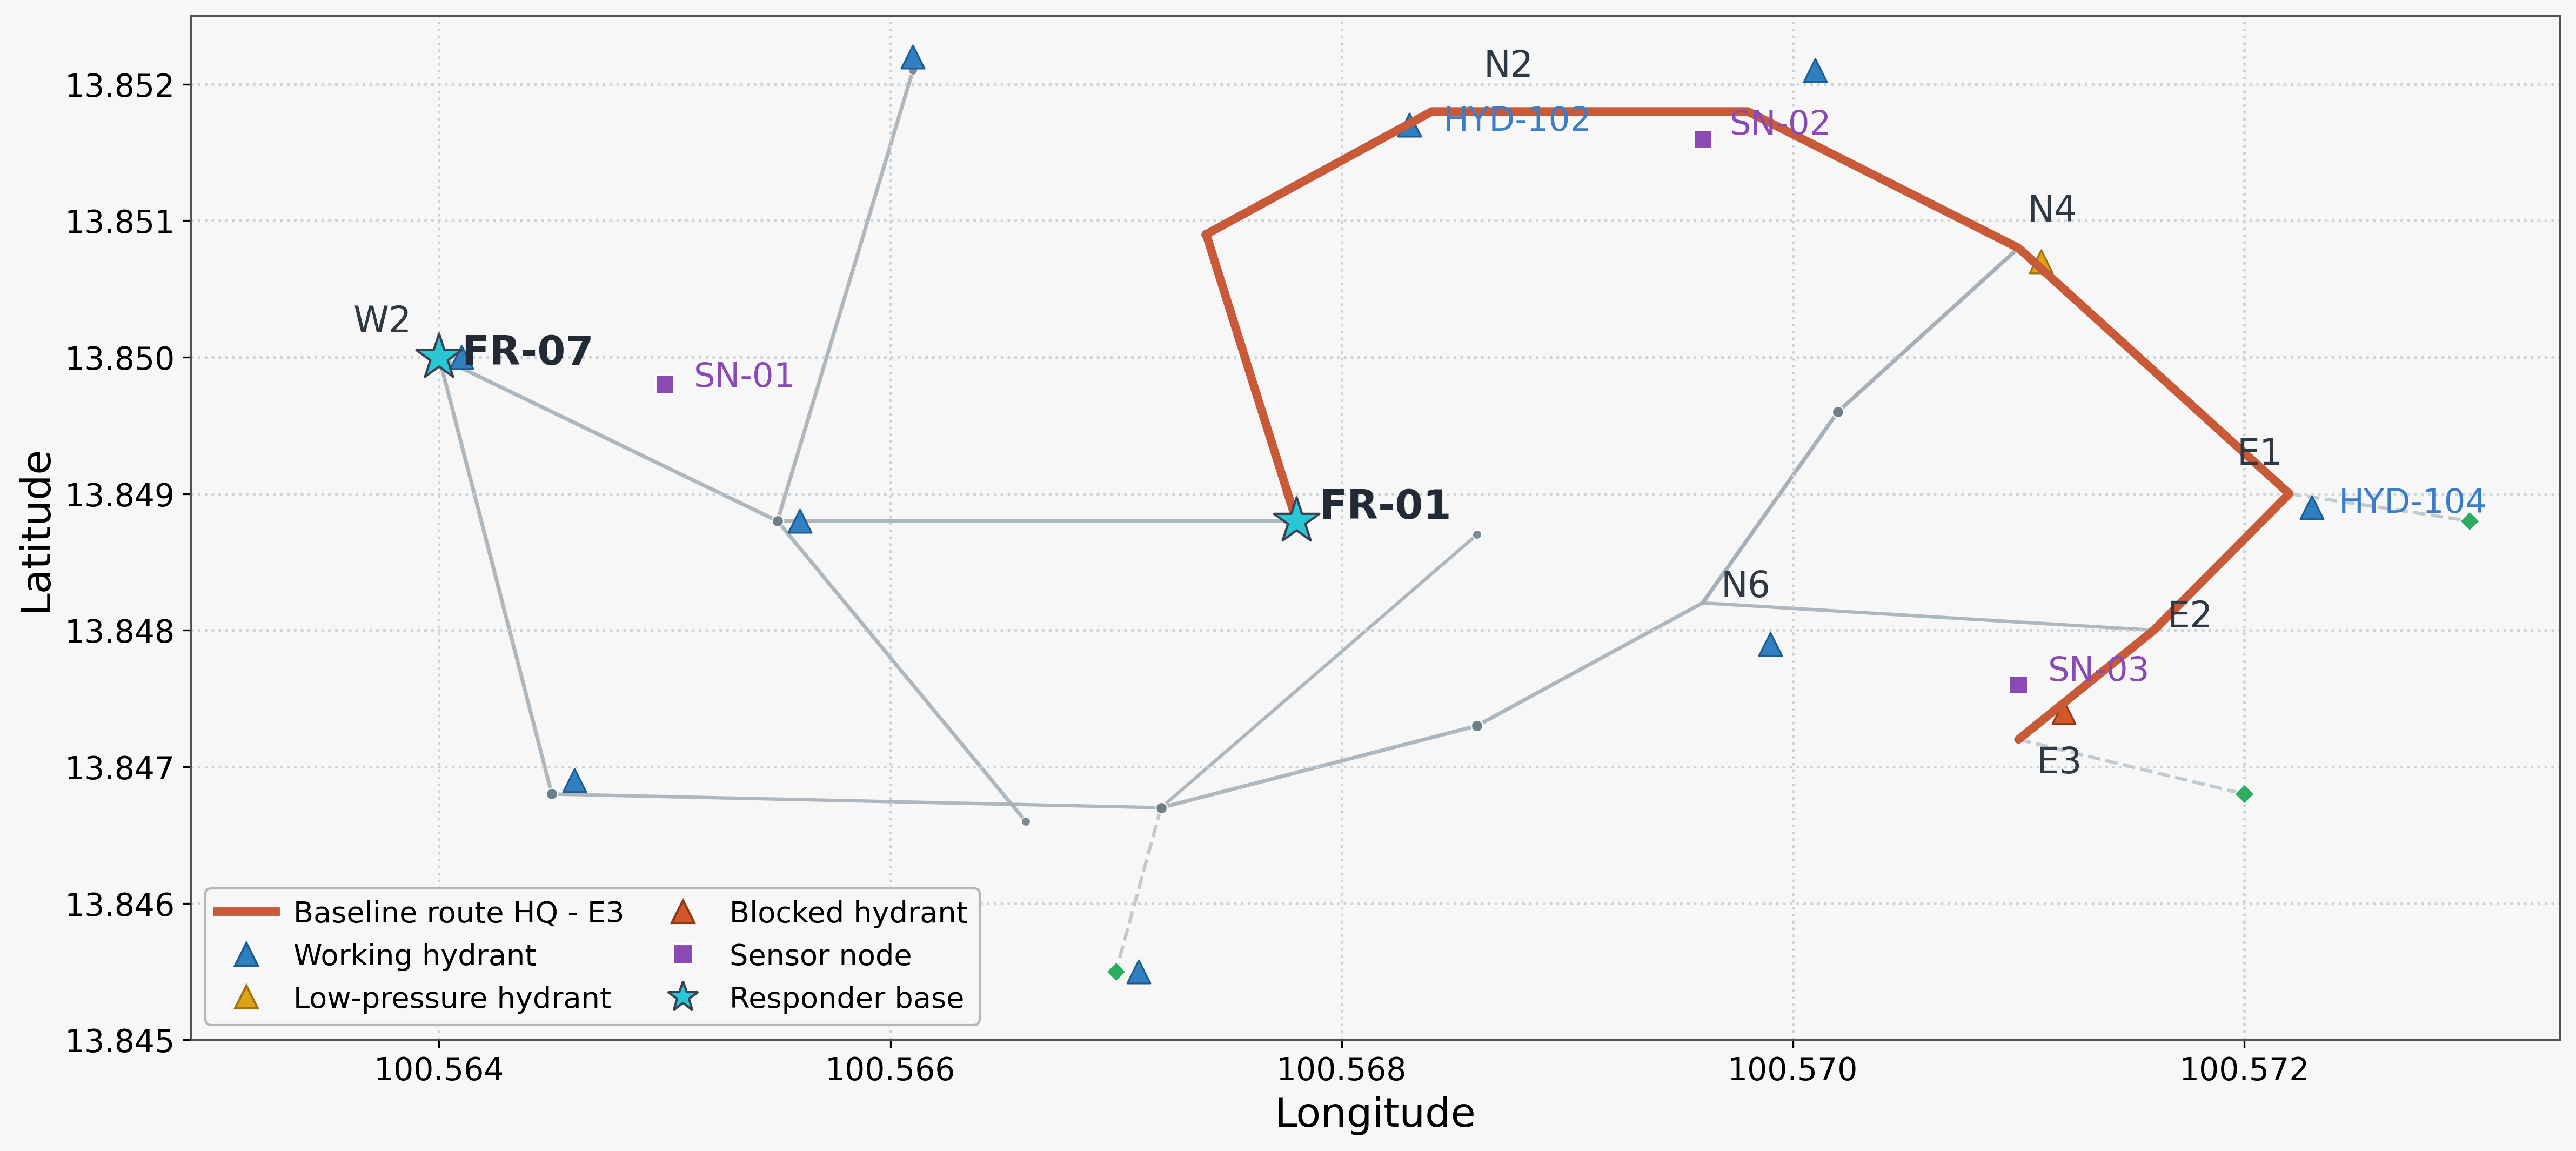
\includegraphics[width=\textwidth]{figure2_pilot_map}
    \caption{Pilot graph and baseline eastern-corridor route reproduced from the package configuration, with hydrants, sensor nodes, and responder bases overlaid from the externalized asset files.}


    \label{fig:pilotmap}
\end{figure*}


\subsubsection{Ablation interpretation}
The ablation study provides detailed insight into the role of each modeling component and its contribution to overall system behavior. By selectively disabling individual factors, we can isolate how specific assumptions influence routing decisions, dispatch outcomes, and system interpretability.

Removing the smoke penalty collapses the difference between the \texttt{smoke\_e3\_08} scenario and the baseline, confirming that environmental degradation acts as a dominant driver of route cost variation. This indicates that the system appropriately captures the impact of dynamic environmental conditions, such as reduced visibility and maneuverability, on operational feasibility. In contrast, removing alley penalties reduces sensitivity to narrow-access constraints, demonstrating that structural factors contribute to routing behavior but exert a comparatively smaller effect than environmental conditions.

Allowing non-\textit{WORKING} hydrants into the candidate set reduces nominal dispatch cost in some scenarios, but leads to operationally unrealistic recommendations. This highlights the importance of infrastructure filtering in ensuring that optimization results remain grounded in real-world feasibility. Similarly, removing blocked-edge infeasibility allows routing through disrupted corridors, effectively suppressing fragility signals and masking critical vulnerabilities in the network. This behavior underscores the importance of explicitly modeling infeasibility to reveal structural weaknesses rather than obscuring them.

Figure~\ref{fig:pilotmap} provides a spatial visualization of the pilot graph and baseline routing behavior. It illustrates how routing decisions interact with the physical layout of the environment, including the placement of hydrants, sensor nodes, and responder bases. This visual representation helps contextualize how constraints such as blocked corridors or narrow access paths influence feasible routes and system behavior. Table~\ref{tab:scenarios} presents a quantitative summary of scenario-based outcomes, including direct travel time, hydrant selection, and overall chain cost. The table highlights how different perturbations systematically affect routing efficiency and resource allocation, making it easier to compare the relative impact of environmental and structural factors across scenarios.

Our ablation results demonstrate that each modeling component contributes meaningfully to system performance. Rather than simply computing shortest paths, the proposed framework encodes operational assumptions that govern sensitivity to environmental conditions, adherence to infrastructure constraints, and interpretability of decision outcomes.


\
